\documentclass[a4,11pt]{article}
\usepackage[a4paper,left=2.54cm,right=2.54cm,bottom=3cm,top=3cm,text={18cm,20cm},footskip=32pt]{geometry}
\usepackage{latexsym} 
\usepackage{amsmath} 
\usepackage{amsthm}	% per la stilizzazione dei teoremi e per gestire extra simboli matematici, size, space, font, etc..
\usepackage{amsopn}	% per stilizzazione di alcuni operatori matematici (e.g. lim e log)
\usepackage{amscd}	% per gestire frecce e circolarità tramite frecce su più livelli in un'equazione (tipo grafi)
\usepackage{amssymb} % per i simboli matematici
\usepackage{array}	% per creare e gestire array
\usepackage{actuarialsymbol} % per simboli attuariali e di matematica finanziaria 
\usepackage{mathtools} 
\usepackage{makeidx} 
\usepackage{multicol} 
\usepackage{multirow} 
\usepackage{caption} 
\usepackage{float} 
\usepackage{enumerate} 
\usepackage{graphicx}  
\usepackage{subfig} 
\usepackage{booktabs} 
\usepackage{color} 
\usepackage[english]{babel} 
\usepackage{wasysym}
\usepackage{appendix} % per inserire appendice
\usepackage{longtable}
\usepackage{hyperref}
\usepackage{collref}
\usepackage{microtype} \graphicspath{ {Figures/}} 
\usepackage{lmodern}
\usepackage{soul}
\usepackage{bm}
\usepackage{bookmark}
\usepackage[authoryear]{natbib}
\usepackage[utf8]{inputenc}
\usepackage[T1]{fontenc}
\usepackage{authblk}

\title{Leveraging deep neural networks to estimate age specific mortality from life expectancy at birth}



\author[1]{Andrea Nigri}
\author[2]{Susanna Levantesi}
\author[3,4]{Jos\'e Manuel Aburto}

\affil[1]{\footnotesize Department of Agricultural Sciences, Food, Natural Resources and Engineering, University of Foggia. andrea.nigri@unifg.it}
\affil[2]{\footnotesize Department of Statistics, Sapienza University of Rome. susanna.levantesi@uniroma1.it}
\affil[3]{\footnotesize Leverhulme Centre for Demographic Science, Department of Sociology and Nuffield College at University of Oxford. jose-manuel.aburto@sociology.ox.ac.uk}
\affil[4]{\footnotesize Interdisciplinary Centre on Population Dynamics, University of Southern Denmark}

%\author{Andrea Nigri, Susanna Levantesi, Jos\'e Manuel Aburto}
%\author{Andrea Nigri\\\small Department of Agricultural Sciences, Food, Natural Resources and Engineering, University of Foggia.\\\small andrea.nigri@unifg.it %\and Susanna Levantesi\\\small Department of Statistics, Sapienza University of Rome\\\small susanna.levantesi@uniroma1.it \and 
%Gabriella Piscopo\\\small Department of Economics and Statistical Science, University of Naples Federico II\\\small gabriella.piscopo@unina.it} 
\date{\today}

\begin{document}
	\maketitle
	%\hl{- Add affiliations (mine are: 1) Leverhulme Centre for Demographic Science, Department of Sociology and Nuffield College at University of Oxford, and 2) Interdisciplinary Centre on Population Dynamics, University of Southern Denmark), and correspondence information.\\
	%- Just Before references add a statement on Data and materials availability where you will add the link to the newest version of code and data to replicate our results \\
	%- Then add a contributions statement.\\
	%- Add an acknowledgements subsection to add those that we'll ask to provide comments.\\
	%- Add a funding statement also to acknowledge any funder: mine can be something like JMA acknowledges support from the British Academy Newton International Fellowship NIFBA19/190679 and the Leverhulme Trust Large Centre Grant. \\
	%- I went back to $\log$, is much nicer than the italic one\\
	%- I changed the results section and brought back results for males for the last time window\\
	%- please re-work the abstract with the current version. In Nature there is a nice manual on how to write abstracts\\
	%- Since we are close to the final version, reformat the PDF (positions of figures, consistency, etc)\\
	%- I think one we are ready to submit we should upload this to a preprint, maybe SocArxiv\\
	%-Consider presenting it at the BSPS meeting}
	
\begin{abstract}
Demography has a long standing tradition of developing formal demographic methods and using statistical approaches to indirectly estimating indicators. According to the UN manual,
the term "indirect" qualifies the demographic estimation technique that origins in the fact that such technique produces estimates of certain parameters on the basis of information that is only indirectly related to its value. Indirect methods were developed by different systems of model life tables and by recent improvements of g techniques adopting a method based on the Lee-Carter model, exploit an inverse approach for converting life expectancy forecasting into age-specific death rates.
The aim of this study is to develop an "indirect" methodology, formulating a model leveraging on deep learning algorithms based on neural networks to derive age-specific mortality profiles from observed or predicted life expectancy levels. 
\end{abstract}
	\bigskip
	\begin{flushleft}
		\textbf{Keywords}: Life expectancy, Forecasting, Death rates, Deep Neural Network.
	\end{flushleft}
%	\newpage
	%--------------------------------------------------------------------------------------------
\section{Introduction}
%--------------------------------------------------------------------------------------------
The rise in human longevity over the last two centuries has led to a growing interest in modelling and predicting death rates and life expectancy at birth (hereafter referred too as life expectancy). Reliable estimates of age-specific mortality are essential in the study of health inequalities and well-being between and within countries. However, this task comes with several difficulties including lack of reliable data or stochastic variation in death counts. Because of these difficulties in several countries and sub-populations, the regularities observed in trends of life expectancy have made this indicator appealing to model and predict. A key advantage of modelling life expectancy at birth, or at any age, is that the predictive model deals only with a single indicator that summarizes the overall level of mortality over time, instead of modelling single time series of death rates for each age simultaneously. 

Approaches that forecast life expectancy consider past trends in this indicator and its regularities, such as the linear increase of the best practice life expectancy \citep{OV2002}. Best practice life expectancy refers the highest life expectancy observed in a given year. \citet{Lee2006} exploits this regularity and models the changes in life expectancy as a linear function of the gap with the best practice trend, allowing countries to exceed the best practice levels. In contrast, \cite{TorriVaupel12} model life expectancy linearly including a smooth function that accounts for the gap with the best practice life expectancy constrained to not allowing countries to overtake the best practice line. \cite{Raftery13} introduce a Bayesian hierarchical model to obtain joint probabilistic projections of life expectancy in an international context. This model is currently used by \cite{UN_2019}. More recently, \cite{Nigri19} propose forecasting life expectancy based on recurrent neural networks. These approaches forecast males and females independently. \cite{Pascariu18} further include the well documented female advantage on longevity \citep{luy2003causes} to forecast life expectancy for both sexes simultaneously. Although the use of life expectancy as an indicator to forecast is appealing, estimating age-specific death rates is needed to analyze patterns of mortality at different ages and to calculate other indicators such as lifespan inequality, as well as for estimating insurance pricing and pension liabilities. This has become even more important with recent patterns of stalls in longevity improvements, or temporary reversals, observed in several countries including the USA and the UK \citep{mehta2020us,aburto2020EstimatingBurdenCOVID19,Ho}, but also around the globe in contexts where timely data is needed and often reported with significant delays such as Mexico or Venezuela \citep{aburto_16,garcia_19}.

Here we propose a model to derive age-specific mortality from observed or predicted life expectancies. The model leverages on deep learning algorithms based on neural networks to uncover age specific mortality based on past trends. Our model is akin to Demography's long tradition of developing formal demographic methods and using statistical approaches to indirectly estimate indicators, such as model life tables \citep{UN_1955,UN_1967,murray2003}, Brass’ relational model \citep{brass1968,brass1971}, the two-dimensional mortality model \citep{wilmoth2012}, and more recently the SVD-Comp approach \citep{clark2019GeneralAgeSpecificMortality}. Two approaches to deriving age-specific mortality from values of life expectancy that are more closely related to ours, which we describe in depth in the next section, were recently proposed by \cite{Sevcikova} and \cite{PascariuLL}. \cite{Sevcikova} adopts a reverting process based on the Lee-Carter model, while \cite{PascariuLL} follow a similar strategy expressing the logarithm of the age-specific deaths as a linear function of the logarithm of life expectancy. 

In this article, we take advantage of deep neural network models to derive the full age-specific mortality profile from values of life expectancy overcoming the linearity assumption from past methods and providing new insights into the indirect approaches. Resulting estimates would be useful for guiding public health interventions, informing about age-specific mortality dynamics in contexts with deficient data collection, as well as pension and social security schemes which rely on longevity dynamics. 



%--------------------------------------------------------------------------------------------
\section{Models to derive age specific mortality from life expectancy}
%--------------------------------------------------------------------------------------------

 \cite{Sevcikova} and \cite{PascariuLL} proposed two models aimed at deriving age-specific mortality from values of life expectancy at birth in line with the functional form of the well known Lee-Carter model \citep{LC1992} given by 
 
 %
	\begin{equation} 
	\label{eq.Lee-carter}
	\log{\left(m_{a,t}\right)}=\alpha_{a}+\beta_{a} \kappa_{t} + \epsilon_{t,a}, 
	\end{equation}
%

where $m_{a,t}$ is the central death rate at age $a$ and time $t$, $\alpha_{a}$ captures the log-mortality average by age, $\kappa_{t}$ is the level of mortality in year $t$, $\beta_{a}$ is an age-pattern of mortality change at age $a$, and $\epsilon_{t,a}$ is the error term. The following constraints on $\kappa_{t}$ and $\beta_{a}$ avoid identifiability problems with the parameters:

\,
$$\sum_{t \in \mathcal{T}}{\kappa_{t}}=0 \quad \sum_{a \in \mathcal{A}}{\beta_a}=1.$$
\,

\citet{LC1992} found that $\kappa_{t}$ changes linearly and can be forecasted using a random walk with drift or other time series methods.

\subsection{ \v{S}ev\v{c}\'{i}kov\'{a} and colleagues model}

The first method proposed to estimate an age specific mortality profile from a projected or forecasted value of life expectancy at birth was developed by \cite{Sevcikova}. Their method consists on calibrating the parameter that reflects the level of mortality in the Lee-Carter model ($\kappa_{t}$) to derive a desired level of life expectancy, similarly to ideas proposed by \cite{lee01} and \cite{li2013}. 

Let $t \in\{1, \ldots, T\}$ and $\tau \in\left\{T+1, \ldots T_{p}\right\}$ denote the observed and projected time periods, respectively. \cite{Sevcikova} estimate the Lee-Carter parameters $\alpha_{a}$, $k_t$ and $\beta_{x}$ using the observed death rates $m_{a,t}$ independently by sex. For a given value of projected life expectancy at birth $e_{0}(\tau)$, the method solves for future $k_{\tau}$ based on the previously estimated parameters $\hat{\alpha}_{a}$ and $\hat{\beta}_{a}$ using life tables. Finally, the age specific log-death rates are derived as
\begin{equation*} 
	\log{\left(m_{a,\tau}\right)}=\hat{\alpha_{a}}+\hat{\beta_{a}} \hat{k_{\tau}}.
\end{equation*}

\subsection{Linear-Link model}

The Linear-Link model proposed by \citet{PascariuLL} derives specific death rates at time $t$ and age $a$, $m_{a,t}$, as a linear function of the logarithm of life expectancy at birth ($e_{0,t}$) at time $t$ given by

	%
	\begin{equation}
	\label{eq.LinearLink}
	\begin{array}{l}
	\log{\left(m_{a,t}\right)}=\beta_{a} \log(e_{0,t})+\nu_{a} k+\varepsilon_{a,t}.
	\end{array}
	\end{equation}
	%
	
The Linear-Link model is based on the least squares estimation of the slope $\beta_a$ over the observation period. $\beta_a$ can be regarded as an age-specific parameter and $\varepsilon_{a,t}$ denotes a set of normally distributed errors with mean zero and variance $\sigma^{2}$. The model specification involves a second step computing the singular value decomposition (SVD) of the matrix of regression residuals to obtain the parameter $\nu_{a}$. To avoid projecting age specific noise, \citet{PascariuLL} smooth the parameters $\beta_{a}$ and $\nu_{a}$ using splines. Finally, the parameter $k$ is optimized to achieve the value of a projected life expectancy. The model can also be estimated assuming that deaths follow a Poisson distribution with maximum likelihood estimation. 


%--------------------------------------------------------------------------------------------
\section{Data}
%--------------------------------------------------------------------------------------------
We use high quality 1$\times$1 life tables from the Human Mortality Data Base \citep{HM} by sex for Japan, the USA, Italy and Russia from 1950 to 2015 to test the accuracy of our model. This set of countries covers a range of longevity trajectories with Japan as one of the highest life expectancies in the world, the USA with stagnation and slow improvements in life expectancy, Italy with its late demographic transition and rapid increase in life expectancy, and Russia with the highest mortality at younger ages and lower life expectancy within the HMD.

%--------------------------------------------------------------------------------------------
\section{Method: Deep Neural Networks}
\label{sec:2}
%--------------------------------------------------------------------------------------------

Machine learning techniques, including deep neural networks (DNN), have become important in a wide range of applications such as image classification or speech recognition with high predictive accuracy, often on par with human performance. However, its applications in demographic research are still scarce. A DNN is a collection of neurons organized in a sequence of multiple layers, where the input is the neuron activation from the previous layer, that performs a weighted sum of the input followed by a nonlinear activation \citep{MONTAVON20181}. The neurons then implement a complex nonlinear mapping from the input to the output. This mapping is learned from the data by adapting the weights of each neuron performing a technique known as error back-propagation \citep{Rumelhart}. The general idea is that for a given set of training data $\left\{\left(x_{1},y_{1}\right) \ldots\left(x_{n},y_{n}\right)\right\}$ sampled according to an unknown probability distribution $\mathrm{P}(\mathbf{x}, 
 \mathbf{y})$, we find a function $\mathrm{f(\cdot)}$ that minimizes the expected error on a new test set of data
 $$
\int \mathrm{L}(\mathrm{y}, \mathrm{f}(\mathbf{x})) \mathrm{P}(\mathbf{x}, \mathbf{y}) \mathrm{d} \mathrm{x} \mathrm{dy},
$$
 where $\mathrm{L}(\mathbf{y}, \mathrm{f}(\mathbf{x}))$ is the loss function that measures the prediction error for a given $x$ against the actual value $y$. We propose a model based on DNN that assigns to life expectancy at birth at time $t$ a vector of age specific death rates with the structure shown in Figure \ref{fig:NN}.

\begin{figure}[H]
\centering
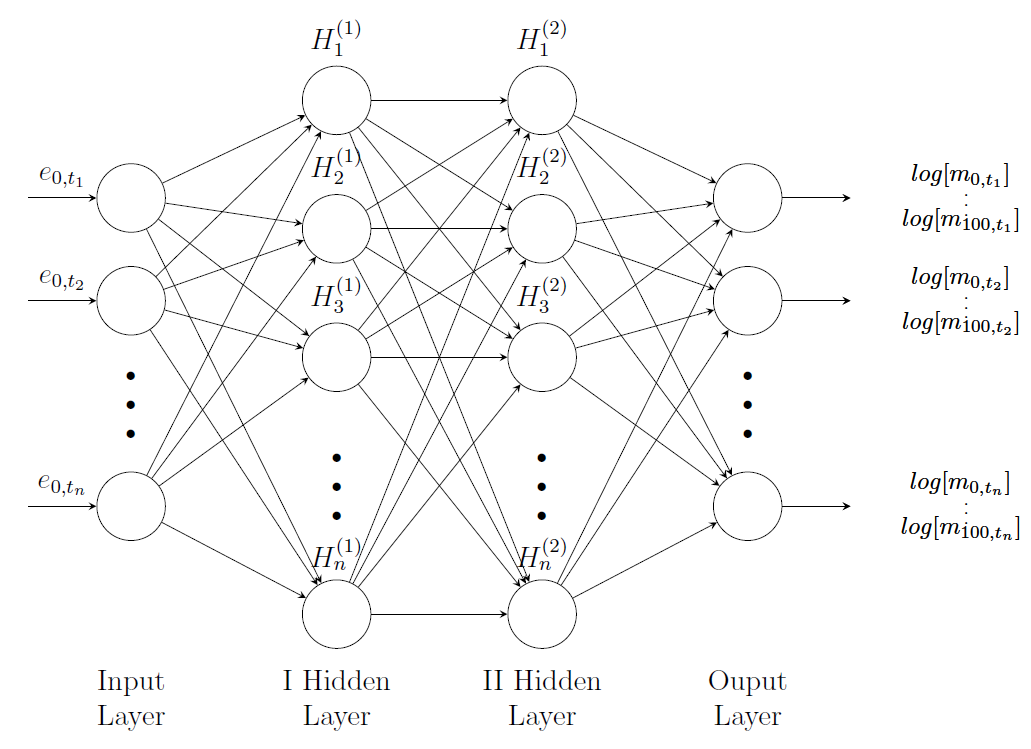
\includegraphics[width=0.8\linewidth]{NNmodel.png}
\caption{\footnotesize Graphical representation of our DNN model. The input is a vector of life expectancies over time $e_{0,t}$, that passes through the neurons and all multiple layers. The output in this diagram is a set of log-death rates at each age that correspond to each value of life expectancy trained with observed age-specific data.}
\label{fig:NN}
\end{figure}

%\hl{Instead of defining $\mathbf{M}=(m_{a,t})_{a\in A,t\in T}$, I think notation would become easier if you define it as $\mathbf{M}=\log(m_{a,t})_{a\in A,t\in T})$. This will eliminate all the 'log' in the following equations and it means the same, please change this.}
Let $\mathbf{M}=\log(m_{a,t})_{a\in A,t\in T}$ be a matrix with death rates, where rows denote age and columns calendar years, and $\mathbf{e_{0}}=(e_{0,t_1},e_{0,t_2},...,e_{0,t_n})$ a vector with corresponding values of life expectancy at birth over time. We set $A=\left\{0,1,...,100\right\}$ and $T=\left\{t_1,t_2,...,t_n\right\}$. Then, for a hidden layer $\mathbf{H}^{(k)}$, the specific neural network structure illustrated in Figure \ref{fig:NN} for the logarithm of death rates is given by

%
\begin{equation}
\mathbf{M} =
%\begin{bmatrix}
%log[\mathbf{m_{(a,t_1)}}] \\
%log[\mathbf{m_{(a,t_2)}}] \\
%log[\mathbf{m_{(a,t_3)}}]\\
%\vdots   \\
%log[\mathbf{m_{(a,t_n)}}] \\
%\end{bmatrix}
f^{(k)} \left(
\begin{bmatrix}
w^{(k)}_{1,1} & w^{(k)}_{1,2} &w^{(k)}_{1,3} & \cdots & w^{(k)}_{1,n} \\
w^{(k)}_{2,1} & w^{(k)}_{2,2} &w^{(k)}_{2,3} & \cdots & w^{(k)}_{2,n} \\
w^{(k)}_{3,1} & w^{(k)}_{3,2} &w^{(k)}_{3,3} & \cdots & w^{(k)}_{3,n} \\
\vdots & \vdots & \vdots & \ddots & \vdots \\
w^{(k)}_{n,1} & w^{(k)}_{n,2} &w^{(k)}_{n,3} & \cdots & w^{(k)}_{n,n} \\
\end{bmatrix}
\begin{bmatrix}
H^{(k-1)}_{1} \\
H^{(k-1)}_{2} \\
H^{(k-1)}_{3} \\
\vdots   \\
H^{(k-1)}_{n} \\
\end{bmatrix}
+
\begin{bmatrix}
b^{(k)}_{1}\\
b^{(k)}_{2} \\
b^{(k)}_{3} \\
\vdots   \\
b^{(k)}_{n} \\
\end{bmatrix}
\right).
\label{eq:1}
\end{equation}
%

where $f^{(k)}$ is the activation function, $\mathbf{W^{(k)}}$ the matrix of weights , $\mathbf{H^{(k-1)}}$ the hidden layers, and $\mathbf{b^{(k)}}$ the bias used to control the triggering value of the activation function. We use the rectified linear unit function given by $f(z)= \max(z, 0)$ \citep{Glorot}. This function ensures faster learning in networks with many layers. In the feed-forward architecture each hidden layer involves the previous one as

%
\begin{equation*}
\mathbf{H^{(k)}}=f^{(k)}\big(\mathbf{W^{(k)}}\,\mathbf{H^{(k-1)}}+\mathbf{b^{(k)}}\big),
\end{equation*}
%

where $\mathbf{H^{(k-1)}}$ can be expressed as a function of a vector with life expectancy values as follows

%
\begin{equation*}
\mathbf{H^{(k-1)}} = f^{(k-1)} \big(\dots f^{(1)}\big(\mathbf{W^{(1)}}\,\mathbf{e_{0}}+\mathbf{b^{(1)}}\big)\dots\big).
\end{equation*}
%

For example, for a standard architecture consisting of three hidden layers $k=3$ (input, hidden and output layer respectively), the theoretical relationship defining the matrix of mortality $\mathbf{M}$ given the vector of life expectancy at birth $\mathbf{e_{0}}$ is represented by

%
\begin{equation}
\label{eq:2}
\mathbf{M}= f^{(3)} \big(\mathbf{W^{(3)}}(f^{(2)}(\mathbf{W^{(2)}}f^{(1)}\big(\mathbf{W^{(1)}}\,\mathbf{e_{0}}+\mathbf{b^{(1)}})+\mathbf{b^{(2)}})+\mathbf{b^{(3)}}),
\end{equation}
%

where $f^{(1)}\big(\mathbf{W^{(1)}}\,\mathbf{e_{0}}+\mathbf{b^{(1)}}\big) = \mathbf{H^{(1)}}$ is the first hidden layer that accepts the vector $\mathbf{e_{0}}$ as input. 

The DNN model is based on a training algorithm that involves an unconstrained optimization problem aiming to minimize the prediction error. The idea is to adjust the weights of the network connections to minimize a measure of the difference between the actual and the desired output ($\mathbf{M}$ and $\mathbf{\hat{M}})$, respectively), known as the loss function $\mathcal{L}$. We use the Mean Square Error (MSE) as a loss function given by

%
$$\mathcal{L}[\mathbf{M},\mathbf{\hat{M}}] = \frac{1}{a \cdot t}\sum_{a,t}\left[\log({m_{a,t}})- \log({\hat{m}_{a,t}})\right]^2$$
%

We chose the MSE because it is the benchmark in neural network regression problems \citep{lecun2015}, and it was the best performer compared to other suitable loss functions with our dataset. To minimize the loss function, we use gradient descent optimization. Gradient descent is one of the most popular algorithms to perform optimization and the most common way to optimize neural networks. It consists on minimizing the loss function by updating the weights in the opposite direction of the gradient ($\nabla \mathcal{L}$) with respect to the weights. For a generic set of weights $w_{n,n}^{(k)}$ and the $k$-th layer, using the chain rule, the gradient is given by

%
\begin{equation}
\label{eq:gradient}
\nabla \mathcal{L} = \frac{\partial \mathcal{L}[\mathbf{M},\mathbf{\hat{M}}]}{\partial w_{n,n}^{(k)}} =\frac{\partial \mathcal{L}[\mathbf{M},\mathbf{\hat{M}}]}{\partial H_n^{(k)}}\,\frac{{\partial H_n^{(k)}}}{\partial z_n^{(k)}} \, \frac{\partial z_n^{(k)}}{\partial w_{n,n}^{(k)}},
\end{equation}
%

where $ z_n^{(k)}=w_{n}^{(k)}\,H_{n}^{(k-1)}+b_n^{(k)}$. The gradient encodes the relative importance of each weight and bias. The algorithm for computing the gradient in equation \eqref{eq:gradient} efficiently is known as back-propagation. Back-propagation consists in a recursive algorithm. In the forward step, the prediction is computed fixing the weights, subsequently, in the backward step, the weights are adjusted by back-propagating the gradient of the loss function to reduce the error. As a result of these adjustments the internal hidden layers, which are no part of the input or output, are able to represent and capture important features of age specific mortality. To update the weights ($\tilde{\mathbf{W}}$), the gradient of the loss function is multiplied by a scalar, $\eta$, often called learning rate, according to the following scheme

%
\begin{equation}
\tilde{\mathbf{W}} = \mathbf{W}-\eta \nabla \mathcal{L} \left[\mathbf{M},\mathbf{\hat{M}}\right]
\end{equation}
%

The learning rate $\eta$ determines the size of the step taken to reach a global or local minimum. In other words, gradient descent is similar to “climbing down a hill” until a global or local minimum is reached. For this stage, we implement the Root Mean Square Propagation (RMSProp) algorithm proposed by \cite{hinton2012neural}.

\subsection*{Implementation}
Our model requires an input vector with the time series of life expectancy at birth and a matrix with the corresponding age specific deaths rates over rows and time periods over columns. Each data series is split into a training-validation set with which the network is trained, and a test set to check the accuracy of the model's prediction. The scheme is presented in Figure \ref{fig:scheme}.

\begin{figure}[H]
	\centering
	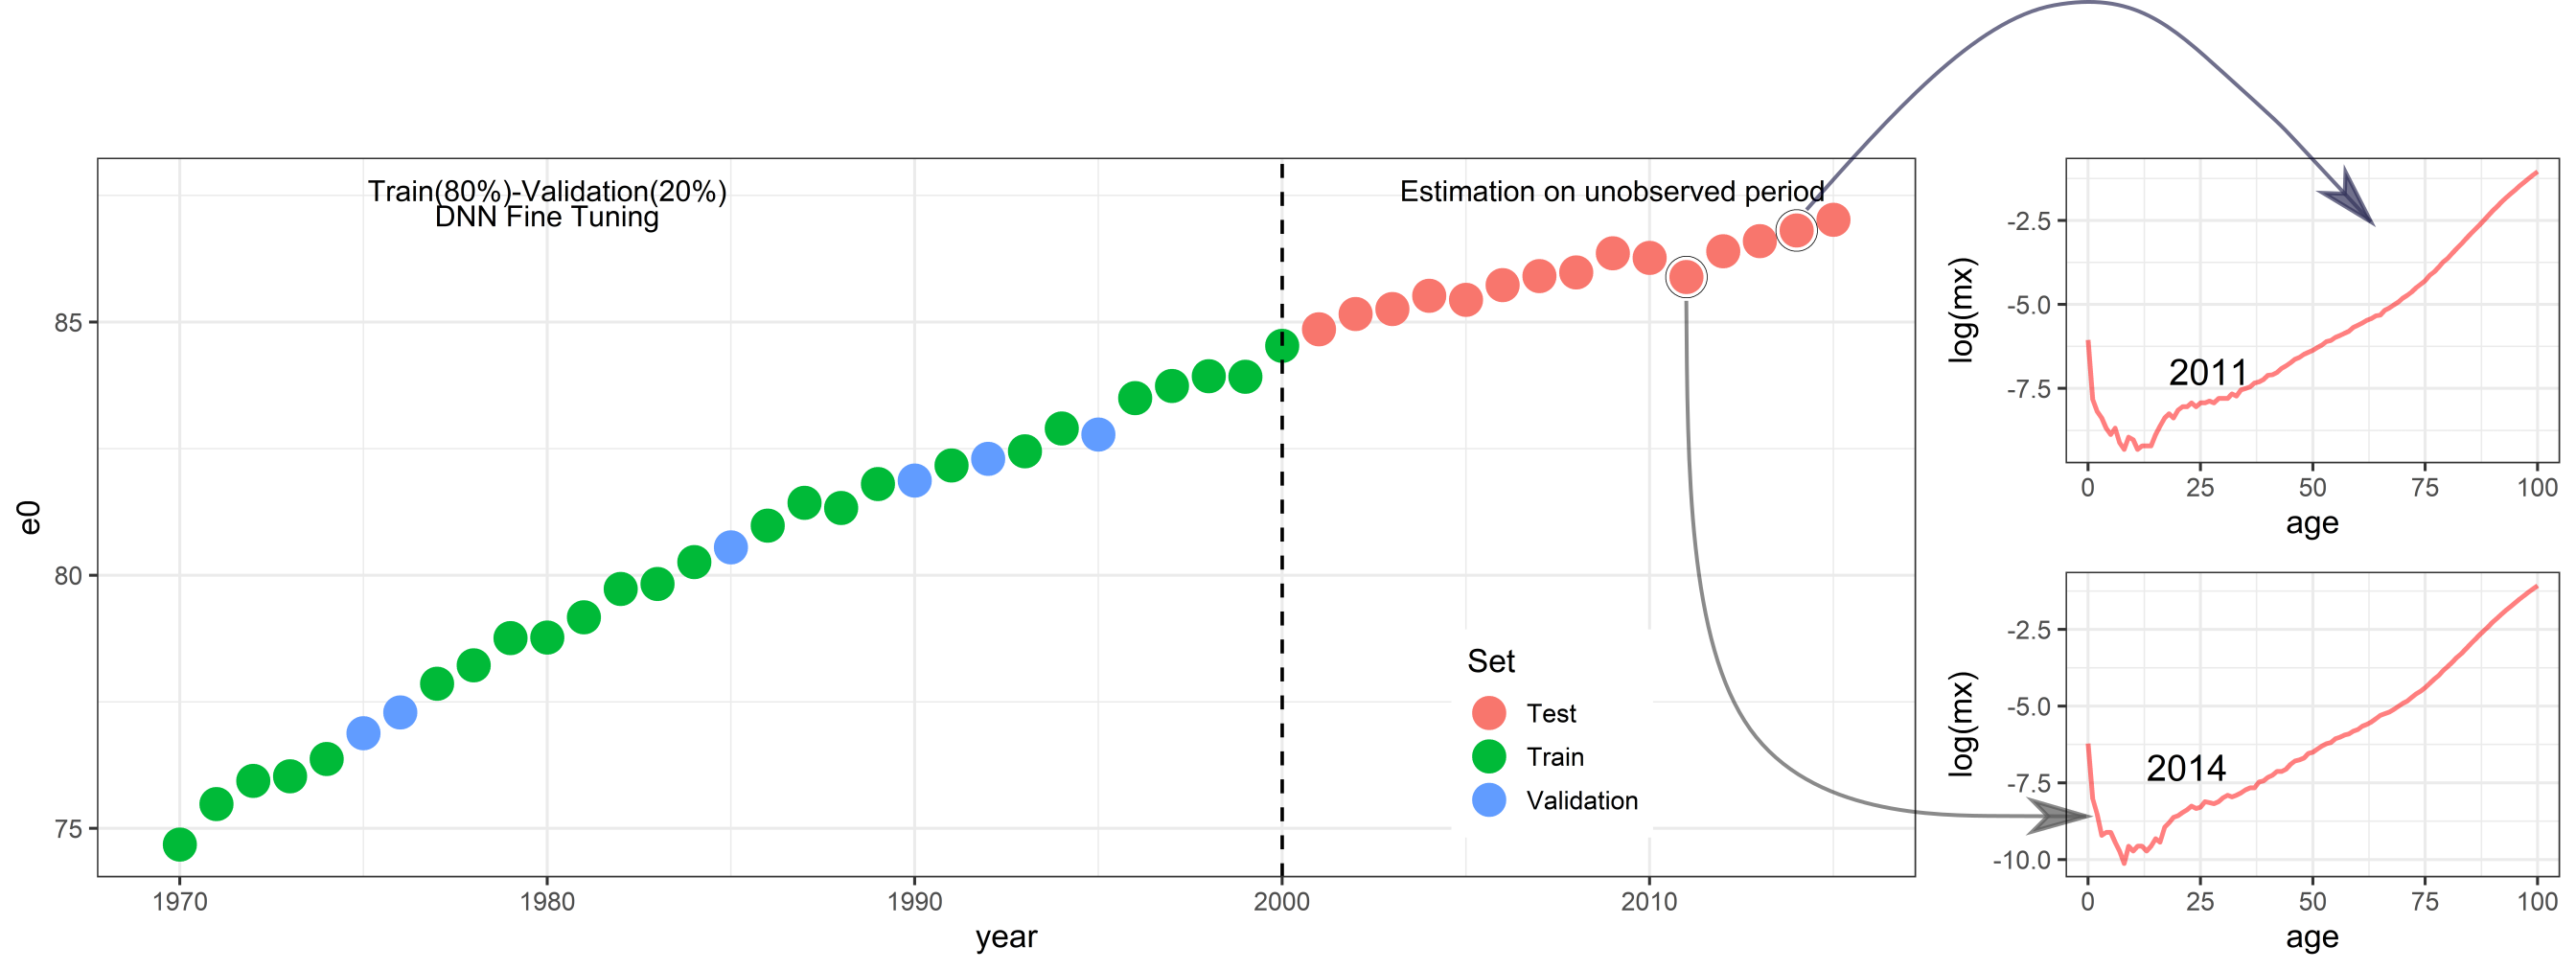
\includegraphics[width=1\linewidth]{tr_val_ts}\\
	 \caption{Scheme of implementation of DNN model. The model is trained and validated with observed age-specific death rates that are consistent with life expectancy levels from the train and validation period (green and blue dots). Results from this training phase are then applied to estimate a full age-specific mortality profile given (projected or forecasted) life expectancy value (orange dots).}
	 \label{fig:scheme}
\end{figure}

To select the optimal number of hidden layers, neurons and parameters used in the DNN, it is common practice to perform a preliminary phase of fine-tuning. The aim of this phase is to choose an appropriate structure of the model (number of hidden layers, neurons) according to the training error minimization. This choice depending on the type of data remains a heuristic problem in the field of neural networks. The process consists on feeding the model the training set and subsequently assess its accuracy on the validation set. The test set stands for the unobserved time horizon, on which the model comparison will be performed. In practice, the test set would be the forecasted or projected life expectancy for which the age-specific mortality profile is unknown. Formally, let $t_{\tau}$, with $t_0<t_{\tau}<t_s$, be the calendar year corresponding to the last realization in the train-validation set. The values of life expectancy in the period $(t_0,t_{\tau})$, $(e_{0,t})_{t\in [t_{0},t_{\tau}]}$, represent the input for train-validation, while the corresponding output is $(\hat{m}_{a,t})_{a\in A,t=[t_{0},t_{\tau}]}$. During the train-validation phase, the neural network weights are estimated and subsequently used in the test phase concerning the period $[t_{\tau+1},t_{s}]$, which start from $t_{\tau+1}$. The resulting DNN estimate is a point estimation, not providing any information on the uncertainty given by $\hat{\mathbf{W}}$. This is one of the main limitations of deep learning algorithms, where the estimation of prediction intervals is still considered a big challenge (\cite{Khosravi} and \cite{Keren}). However, in our problem, an alternative is to perform the model on the lower and upper bound of the forecasted/projected life expectancy as pseudo confidence intervals providing a measure of uncertainty.  

%--------------------------------------------------------------------------------------------
\section{Results}
%--------------------------------------------------------------------------------------------

To assess the robustness of our method, we performed an out-of-sample test over three time windows (1950-1980, 1960-1990, and 1970-2000) used as train-validation sets (split according to the 80\%-20\% splitting rule randomly sampled), and the subsequent years of each time window (1981-1995, 1991-2005 and 2001-2015 respectively) as test sets. The model was applied to data from Italy, Japan, Russia and the USA by sex. We use a six hidden-layers architecture following the fine-tuning phase. We compare results from the DNN model with those obtained with the \citet{Sevcikova} and Linear-Link models. To ensure comparability, results were smoothed using P-splines (\cite{HeNg}).\footnote{Unsmoothed results are shown in the additional material. The smoothing step does not affect the models' accuracy ranking: the RMSE and MAE improvements after the smoothing are on average 1.55\% and 1.57\%, respectively.}  We focus on results pertaining to females during the period 2001-2015 in this section, results related to males in the same years and in the other study periods for both genders are reported in the Appendix Section \ref{appendix:a}. 

\subsection*{Age-specific mortality estimates}

Figure \ref{fig:estimate.age.mx} shows age specific deaths rates (in log scale) for females in Russia, Japan, Italy, and the USA. The observed (target) profile is shown with dots and estimated values from the models using the training period 1970-2000 correspond to DNN (red line), Linear-Link (green), and \citet{Sevcikova} (blue). The three models capture the general pattern of mortality, with decreasing trend from birth to around age 15, and increasing linearly from around age 30. For Italy and recent period in Russia, the \citet{Sevcikova} model tends to overestimate mortality at young ages, while the opposite is true for the Linear-Link in the case of Japan. The DNN model captures well the mortality patterns. The three models fail to capture the sharp decrease from infancy accurately in the cases of Italy and Russia.

\begin{figure}[H]
	\centering
	\includegraphics[width=1\linewidth]{age_pattern_F_1970}\\
	 \caption{Estimated age-specific female log-mortality rates $\log(m_{a,t})$ for three models: DNN, Linear-Link and \citet{Sevcikova}, by country for 2005, 2010 and 2014 based on training period 1970-2000. Black dots are the observed log-mortality rates.} 
	 \label{fig:estimate.age.mx}
\end{figure}



\subsection*{Age-specific relative differences} 


We further analyze the accuracy of the models with the relative differences ($\Delta_{a,t}$) between estimates and the observed death rate by age for each model defined as (see Figure \ref{fig:relative.diff})

$$\Delta_{a,t}=\frac{\log(\hat{m}_{a,t})-\log(m_{a,t})}{\log(m_{a,t})}.$$

Because the relative difference is calculated from the log-death rates, red hues indicate that the model underestimates mortality, while blue hues indicate overestimation. Differences with the observed mortality profile are small in general across models and countries. It is observed a systematic underestimation in working-ages (20-50) for Russia and USA from the DNN and Linear-Link models in the time window 2001-2015 (the other two time windows are shown in the Appendix Figures \ref{A:1}, \ref{A:2} , \ref{A:3} , \ref{A:4}). Similarly, there is increased deviation at very old ages for recent periods from both models. In contrast, the \citet{Sevcikova} model tends to overestimate mortality at older ages for all countries, especially for recent periods in Russia. 

\begin{figure}[H]
	\centering
	\includegraphics[width=0.8\linewidth]{final_Heatmap_F_1970}\\
	 \caption{Relative differences ($\Delta_{a,t}$) between estimates and the observed death rate by age for each model. Red hues indicate that the model underestimates mortality, while blue hues indicate overestimation. Females, test period: 2001-2015.}
	 \label{fig:relative.diff}
\end{figure}

Among males (Figure \ref{fig:relative.diff.MALE}, the DNN model and the Linear-Link tend to underestimate mortality at working-ages, which is compensated with increased mortality at younger and older ages below age 90. In contrast, the \citet{Sevcikova} model, as in the case for females, tends to overestimate mortality across all countries, but is the best to capture the working-age pattern for Russia and USA. Notably, deviations from the observed mortality increase with time across all time windows.

\begin{figure}[H]
	\centering
	\includegraphics[width=0.8\linewidth]{final_Heatmap_M_1970}\\
	 \caption{Relative differences ($\Delta_{a,t}$) between estimates and the observed death rate by age for each model. Red hues indicate that the model underestimates mortality, while blue hues indicate overestimation. Males, test period: 2001-2015.}
	 \label{fig:relative.diff.MALE}
\end{figure}

\subsection*{Root Mean Square Error (RMSE) and Mean Absolute Error (MAE)}

To summarize the performance of the methods and to evaluate their accuracy we report the Root Mean Square Error (RMSE) and Mean Absolute Error (MAE) on the test sets given by 

\begin{equation*}
	\text{MAE}: \quad \sum^{n} \frac{\mid \log(m_{a,t}) - \log(\hat{m}_{a,t}) \mid}{n},
	\end{equation*}
	\begin{equation*}
	\text{RMSE}: \quad \sqrt{\frac{\sum^{n} (\log(m_{a,t}) - \log(\hat{m}_{a,t})^2}{n}}. 
\end{equation*}

Tables \ref{tab:1} and \ref{tab:2} summarize the MAE and RMSE for the three models and four countries over the three time windows that we study for females and males, respectively. For females, the DNN is the best performer in most cases, although the Linear-Link showed the lowest MAE for Italy in the earliest and latest periods. The \citet{Sevcikova} model exhibited the lowest RMSE for Russia in the period 1991-2005. Results for males (see table \ref{tab:2}) show less consistent results. For Italy and the USA, the DNN model consistently showed the lowest errors, but the \citet{Sevcikova} model performed the best for Japanese males. 

Among males, for Italy and USA the DNN was the best performed in terms of MAE and RMSE. For Japan, as noted in the age-specific figures, the \citet{Sevcikova} model showed the lowest errors. While for Russia, it was a mix between the three models depending on the time window and summary measure. For both sexes, while the DNN showed in the majority of cases the lowest departures from the age-specific mortality, the Linear-Link performed the best in capturing the life expectancy level.


\begin{table}[H]
		\centering
		\caption{Out-of-sample test: MAE and RMSE for DNN, Linear-Link, and \v{S}ev\v{c}\'{i}kov\'{a} et al. 2016 by country and sex. Estimation periods: 1981-1995 (columns 3-4), 1991-2005 (columns 5-6), and 2001-2015 (columns 7-8). Females.}
		\label{tab:1}
			\footnotesize	
		\begin{tabular}{cl|cc|cc|cc}
			\hline 		
			\multirow{2}{*}{\textbf{Country}} & \multirow{2}{*}{\textbf{Model}} & \multicolumn{2}{c|}{\textbf{1981-1995}} & \multicolumn{2}{c}{\textbf{1991-2005}} & \multicolumn{2}{c}{\textbf{2001-2015}}\tabularnewline
			\cline{3-8} 
			& & MAE & RMSE & MAE & RMSE & MAE & RMSE\tabularnewline
			\hline 
			\multirow{4}{*}{\textbf{\textit{Italy}}} & \multirow{1}{*}{DNN} &0.1672& \textbf{0.2017}&\textbf{0.1038}& \textbf{0.1418}&0.1210& \textbf{0.1591} \tabularnewline
			& \multirow{1}{*}{Linear-Link} &\textbf{0.1379}& 0.2325& 0.1561 &0.2272&\textbf{0.1154}& 0.1818 \tabularnewline
      & \multirow{1}{*}{\v{S}ev\v{c}\'{i}kov\'{a} et al. 2016} &0.2421&0.2995& 0.2042 &0.2598& 0.2539& 0.3278 \tabularnewline
      \hline 
			\multirow{4}{*}{\textbf{\textit{Japan}}} & \multirow{1}{*}{DNN} &\textbf{0.1730}& \textbf{0.2055}& \textbf{0.1182}& \textbf{0.1532}&\textbf{0.1137}&\textbf{ 0.1436}\tabularnewline
			& \multirow{1}{*}{Linear-Link} &0.4036& 0.5473& 0.2602& 0.3242&0.1664& 0.2095 \tabularnewline
      & \multirow{1}{*}{\v{S}ev\v{c}\'{i}kov\'{a} et al. 2016}&0.2444& 0.2785 & 0.1906& 0.2376&0.1656& 0.2014 \tabularnewline
      \hline 
\multirow{4}{*}{\textbf{\textit{USA}}} &\multirow{1}{*}{DNN} &\textbf{0.0572}&\textbf{ 0.0788}&\textbf{ 0.0873}& \textbf{0.1119}&\textbf{0.0944}& \textbf{0.1206} \tabularnewline
			& \multirow{1}{*}{Linear-Link} &0.0720 &0.1196& 0.0949 &0.1541&0.1183& 0.1683 \tabularnewline
 	 		&\multirow{1}{*}{\v{S}ev\v{c}\'{i}kov\'{a} et al. 2016} &0.1291 &0.1642& 0.1081 &0.1524&0.1227& 0.1643\tabularnewline
      \hline 
\multirow{4}{*}{\textbf{\textit{Russia (2014)}}} &\multirow{1}{*}{DNN} &-&-&\textbf{0.1714}&0.2544&\textbf{0.1670}& \textbf{0.2393}\tabularnewline
			& \multirow{1}{*}{Linear-Link} &-&-& 0.1942& 0.2736&0.2266& 0.3223 \tabularnewline
 	 		&\multirow{1}{*}{\v{S}ev\v{c}\'{i}kov\'{a} et al. 2016}&-&-& 0.1931& \textbf{0.2510}&0.1907& 0.2558 \tabularnewline
 	 		\hline 
		\end{tabular}
	\end{table}
%


\begin{table}[H]
		\centering
		\caption{Out-of-sample test: MAE and RMSE for DNN, Linear-Link, and \v{S}ev\v{c}\'{i}kov\'{a} et al. 2016 by country and sex. Estimation periods: 1981-1995 (columns 3-4), 1991-2005 (columns 5-6), and 2001-2015 (columns 7-8). Males.}
		\label{tab:2}
			\footnotesize	
		\begin{tabular}{cl|cc|cc|cc}
			\hline 		
			\multirow{2}{*}{\textbf{Country}} & \multirow{2}{*}{\textbf{Model}} & \multicolumn{2}{c|}{\textbf{1981-1995}} & \multicolumn{2}{c}{\textbf{1991-2005}} & \multicolumn{2}{c}{\textbf{2001-2015}}\tabularnewline
			\cline{3-8} 
			& & MAE & RMSE & MAE & RMSE & MAE & RMSE\tabularnewline
			\hline 
			\multirow{4}{*}{\textbf{\textit{Italy}}} & \multirow{1}{*}{DNN} &\textbf{0.1419}& \textbf{0.2203}&\textbf{0.1107}& \textbf{0.1493}&\textbf{0.1194}& \textbf{0.1566} \tabularnewline
			& \multirow{1}{*}{Linear-Link} &0.1840 &0.2846& 0.1993& 0.2780&0.1541& 0.2158 \tabularnewline
      & \multirow{1}{*}{\v{S}ev\v{c}\'{i}kov\'{a} et al. 2016}& 0.1477 &0.2596 &0.1112 &0.1701 &0.1274 &0.1992 \tabularnewline
      \hline 
			\multirow{4}{*}{\textbf{\textit{Japan}}} & \multirow{1}{*}{DNN} &0.1049&\textbf{ 0.1241}& 0.0943&0.1264& 0.0986& 0.1254 \tabularnewline
			& \multirow{1}{*}{Linear-Link} &0.1585 &0.2088& 0.1014& 0.1392&0.1011& 0.1480 \tabularnewline
      & \multirow{1}{*}{\v{S}ev\v{c}\'{i}kov\'{a} et al. 2016}&\textbf{0.1042} &0.1348& \textbf{0.0874}& \textbf{0.1205}&\textbf{0.0684} & \textbf{0.0958} \tabularnewline
      \hline
			 \multirow{4}{*}{\textbf{\textit{USA}}} &\multirow{1}{*}{DNN} &\textbf{0.0746} &\textbf{0.1088}&\textbf{ 0.0730}&\textbf{0.0907}&\textbf{0.0955}& \textbf{0.1127}\tabularnewline
			& \multirow{1}{*}{Linear-Link} &0.1020 &0.1561& 0.1029& 0.1437&0.1029& 0.1367 \tabularnewline
 	 		&\multirow{1}{*}{\v{S}ev\v{c}\'{i}kov\'{a} et al. 2016}&0.07974 &0.1218& 0.0907& 0.1310&0.1085& 0.1437 \tabularnewline
 	 		\hline 
	 \multirow{4}{*}{\textbf{\textit{Russia (2014)}}} &\multirow{1}{*}{DNN} &-&-&0.1989&\textbf{0.2366}&\textbf{0.1497}& 0.2412\tabularnewline
			& \multirow{1}{*}{Linear-Link} &-&-& \textbf{0.1739}& 0.2544&0.1951& 0.3067 \tabularnewline
 	 		&\multirow{1}{*}{\v{S}ev\v{c}\'{i}kov\'{a} et al. 2016}&-&-& 0.2287&0.2940&0.1515& \textbf{0.2246} \tabularnewline
 	 		\hline 

		\end{tabular}
	\end{table}

\section{Multi population Model (mp-DNN)}

The overall longevity dynamics around the globe may be explained by country-specific trends, not easy to handle in a global view, however. Indeed, data dimensionality might easily reach a size difficult to manage and a common solution is to analyze each population separately.
The evolution of life expectancy is not coincidental but a result of a heterogeneous process that embraces historical changes.
Indeed, common features such as socioeconomic similarity, public health improvements, require estimating mortality for these countries as a group, even if the aim is only in forecasts for a single population.
The indirect estimation models we describe, included the ones we use as benchmarks (LL and Sevcikova), are developed to be applied to a single population. Then the models should be estimated on each population separately, in the case of multiple populations estimation was require.
To this end, we provide a further step head, extending our DNN model to multiple populations, i.e. countries, and both genders.

\subsection{mp-DNN}
Starting from the DNN proposed in Section \ref{sec:2}, we still model the functional relationship between life expectancy at birth and death rates, as numerical inputs and outputs. To extend the framework to the multi-population version, adding demographic features, we turn to the embedding layers (\citet{richman}; \citet{embedding}).
Embedding is a tool most well-known as word embeddings, thank its use in natural language processing, where it allows to capture relationships in language that are very difficult to capture otherwise due to the high dimensionality. 
The proposed extension exploits embedding layers, to embed categorical demographic variables, where the features space characterized by country, gender, age, and year, is embedded into a low dimensional vector,  used during the training phase.

\subsection{Results}
Figures \ref{fig:MP.estimate.age.mx_F} and \ref{fig:MP.estimate.age.mx_M}, show age-specific death rates (in log scale) for females and males in Russia, Japan, Italy, and the USA estimated exploiting the mp-DNN framework trained on the whole HMD.
At glance, we can see that mp-DNN provides smoothed estimation by nature, due to a wider training sample. 
The model well describes the general mortality shape, it provides good fits for Italy and Japan, and a remarkable accuracy for  Russia, which represents a real challenge for the single population models.
The USA provides a particular example where mp-DNN constantly underestimates mortality, at both young and older ages.

\begin{figure}[H]
	\centering
	\includegraphics[width=1\linewidth]{MP_age_pattern_M_1970}\\
	 \caption{Estimated age-specific male log-mortality rates $\log(m_{a,t})$ for the mp-DNN model, by country for 2005, 2010 and 2014 based on training period 1970-2000. Black dots are the observed log-mortality rates.} 
	 \label{fig:MP.estimate.age.mx_M}
\end{figure}

\begin{figure}[H]
	\centering
	\includegraphics[width=1\linewidth]{MP_age_pattern_F_1970}\\
	 \caption{Estimated age-specific female log-mortality rates $\log(m_{a,t})$ for the mp-DNN model, by country for 2005, 2010 and 2014 based on training period 1970-2000. Black dots are the observed log-mortality rates.} 
	 \label{fig:MP.estimate.age.mx_F}
\end{figure}

Figures \ref{fig:MP.relative.diff.MALE} and \ref{fig:MP.relative.diff.FEMALE}, provide the accuracy of the mp-DNN model with the relative differences ($\Delta_{a,t}$) between estimates and the observed death rate by age and time windows.
Overall, mp-DNN shows small deviations with the observed mortality profile, across countries and periods, with the exception of the USA both gender. In this case, the model provides inconsistent results, showing underestimations that increase over time.
Italy, in particular the female population, shows high age-specific sensitivity toward periods, shifting from overestimation to underestimation of the older ages.
For Japan and Russia, as noted in the age-specific figures, the model provides reliable estimations, notably, deviations from the observed mortality decrease across all time windows.\\

Tables \ref{tab:3} and \ref{tab:4} show the MAE and RMSE for the Multi-Population model estimation for four countries over the three-study periods for both gender. 
We can confirm the inadequacy of this model to represent the USA mortality dynamics. On the contrary, we bring evidence of good accuracy for Italy and Japan, remarkable results in terms of errors referring to Russia's both genders.
We underline that mp-DNN is able to provide estimation for RUSSIA over the first time window, where other models are not. Indeed, 
single population models, in order to estimate parameters need training data, that are not completely provided for Russia in the reference period 1950-1980. The mp-DNN leverages on the multi-population estimated parameters, applying them to the Russia case on the out-of-sample window (1981-1995).\\

\begin{figure}[H]
	\centering
	\includegraphics[width=0.8\linewidth]{MULTIPOP_final_Heatmap_M}\\
	 \caption{Relative differences ($\Delta_{a,t}$) between estimates and the observed death rate by age for mp-DNN model. Red hues indicate that the model underestimates mortality, while blue hues indicate overestimation. Males, test period: 2001-2015.}
	 \label{fig:MP.relative.diff.MALE}
\end{figure}

\begin{figure}[H]
	\centering
	\includegraphics[width=0.8\linewidth]{MULTIPOP_final_Heatmap_F}\\
	 \caption{Relative differences ($\Delta_{a,t}$) between estimates and the observed death rate by age for mp-DNN model. Red hues indicate that the model underestimates mortality, while blue hues indicate overestimation. Males, test period: 2001-2015.}
	 \label{fig:MP.relative.diff.FEMALE}
\end{figure}

\begin{table}[H]
\centering
\caption{Out-of-sample test: MAE and RMSE for mp-DNN by country and sex. Estimation periods: 1981-1995 (columns 3-4), 1991-2005 (columns 5-6), and 2001-2015 (columns 7-8). Females.}
\label{tab:3}
\footnotesize	
\begin{tabular}{cl|cc|cc|cc}
\hline 		
\multirow{2}{*}{\textbf{Country}} & \multirow{2}{*}{\textbf{Model}} & \multicolumn{2}{c|}{\textbf{1981-1995}} & \multicolumn{2}{c}{\textbf{1991-2005}} & \multicolumn{2}{c}{\textbf{2001-2015}}\tabularnewline
\cline{3-8}  & & MAE & RMSE & MAE & RMSE & MAE & RMSE\tabularnewline
\hline 
\multirow{1}{*}{\textbf{\textit{Italy}}} &  \multirow{1}{*}{mp-DNN} &0.1380 & 0.1827 & 0.1024 & 0.1592 & 0.1395 & 0.1897 \tabularnewline 	 		
\hline 
\multirow{1}{*}{\textbf{\textit{Japan}}} & \multirow{1}{*}{mp-DNN} &0.1707& 0.2026& 0.09544 &0.1215 & 0.09131 & 0.1314 \tabularnewline 	 		
\hline 
\multirow{1}{*}{\textbf{\textit{USA}}} & \multirow{1}{*}{mp-DNN} &0.1462 & 0.177 & 0.107 & 0.1336 & 0.2397 & 0.3115 \tabularnewline 	 		
\hline 
\multirow{1}{*}{\textbf{\textit{Russia (2014)}}} & \multirow{1}{*}{mp-DNN} &0.144 & 0.1728 & 0.1124 & 0.1382 & 0.1003 & 0.1265 \tabularnewline 	 		
\hline 
\end{tabular}
\end{table}

\begin{table}[H]
\centering
\caption{Out-of-sample test: MAE and RMSE for mp-DNN by country and sex. Estimation periods: 1981-1995 (columns 3-4), 1991-2005 (columns 5-6), and 2001-2015 (columns 7-8). Males.}
\label{tab:4}
\footnotesize	
\begin{tabular}{cl|cc|cc|cc}
\hline 		
\multirow{2}{*}{\textbf{Country}} & \multirow{2}{*}{\textbf{Model}} & \multicolumn{2}{c|}{\textbf{1981-1995}} & \multicolumn{2}{c}{\textbf{1991-2005}} & \multicolumn{2}{c}{\textbf{2001-2015}}\tabularnewline
\cline{3-8} & & MAE & RMSE & MAE & RMSE & MAE & RMSE\tabularnewline
\hline 
\multirow{1}{*}{\textbf{\textit{Italy}}}& \multirow{1}{*}{mp-DNN} &0.1276 & 0.1971 & 0.0972 & 0.1659 & 0.1257 & 0.1603 \tabularnewline 	 		
\hline 
\multirow{1}{*}{\textbf{\textit{Japan}}} & \multirow{1}{*}{mp-DNN} &0.117 & 0.1683 & 0.0875 & 0.1232 & 0.08049 &0.1095 \tabularnewline 	 
\hline
 \multirow{1}{*}{\textbf{\textit{USA}}}& \multirow{1}{*}{mp-DNN} &0.2093 & 0.2614 & 0.1451 & 0.1805 & 0.2535 & 0.3038 \tabularnewline 	 		
\hline 
\multirow{1}{*}{\textbf{\textit{Russia (2014)}}}& \multirow{1}{*}{mp-DNN} &0.1356 & 0.1854 & 0.1849 & 0.2267& 0.08918 & 0.1216 \tabularnewline 	 		
\hline 
\end{tabular}
\end{table}

\section{Conclusion}

We presented a novel method to indirectly estimate a full mortality profile from a level of life expectancy at birth leveraging Deep Neural Networks using prior information on age specific mortality. When tested with state-of-the-art methodologies, the DNN model performed the best in many cases with fewer assumptions than previous methods.
The method outlined here is non-parametric, data-driven, and does not rely on assumptions that may not be completely accurate, as in previous models. Nevertheless, the results show that the three models tested here perform in a satisfactory way, with the DNN offering the best performance in most cases. Moreover, all three models require the same data input, which can be difficult to acquire in some settings. As we showed, the reconstruction of an accurate mortality surface from a given level of demographic summary measure such as life expectancy is challenging. However, we offer a new alternative based on machine learning algorithms that complement the existing demographic toolbox. Moreover, the analysis of four countries with substantially different mortality and three sequential time windows of thirty years provided robust results. 
We confirm that only the Linear -Link, because of its dynamic constraint and consequential reparametrization, assures the coherence with respect to input life expectancy level (providing a negligible error). This not hold for the Sevcikova model, and DNN as well, despite its superior performances on mortality rate estimation.

In some cases, a multi population estimate is required, although the LL and Sevcikova models can supposedly be extended to multi-population, this step is not straightforward.
Indeed as in the case of the Lee-Carter multi population, the structure is hard to justify, the parameterization and the relative optimization procedure could be challenging. In this paper, we take a step forward among demographic methods, offering a multi-population indirect estimation based on data driven approach, that can be fitted to many populations simultaneously, using DNN optimization approaches.
While we apply our methodology to country-specific scenarios, the model could be used to indirectly estimate mortality profiles for regions or subpopulations with similar mortality profiles. This characteristic makes our model appealing for countries where present information is lacking but past data are available or from surrounding countries or populations, as we have shown in the Russian case. Similarly, our method can be used to derive age specific mortality for a projected or forecasted value of life expectancy at birth. 

We acknowledge that our model is subject to several limitations, including the choice of the architecture (e.g., the number of hidden layers) and the parameters involved in the training phase. This remains a heuristic problem for neural network users, indeed the choice often depends on the type of data, and a preliminary round of fine-tuning, before the testing, is highly desired which might be time-consuming (\cite{Nigri}). 
This issue is dimmed in the case of multi-population. Indeed, this framework relies on a bigger data set, thus more examples during the training phases, which has twofold implications. 
On one hand, the model provides more robustness toward structural changes; on the contrary, some country-specific dynamics may not be captured, as in the case of the USA. Therefore, we strongly recommend a careful selection of the countries subgroup on which DNN will be trained.\\
To conclude, here we propose a new approach that provides a valuable alternative tool to capture irregular mortality trajectories. While machine learning techniques are not widely used in the field of demography, our method shows that they can be used to provide robust estimations of age-specific death rates. This may foster new research at the frontier of mortality studies using innovative, yet simple to implement, techniques such as the DNN. This is even more important in a context of rapid population aging and fast mortality decline, but also in contexts where mortality estimates are lacking that can provide crucial information for policy planning.


\bibliographystyle{apa}
\bibliography{bibl}

\appendix
\section{Appendix}
\label{appendix:a}
\setcounter{figure}{0}
\counterwithin{figure}{section}

\begin{figure}[H]
	\centering
	\includegraphics[width=0.8\linewidth]{final_Heatmap_F_1960}\\
	 \caption{Relative differences ($\Delta_{a,t}$) between estimates and the observed death rate by age for each model. Red hues indicate that the model underestimates mortality, while blue hues indicate overestimation. Females, test period: 1991-2005.}
	 \label{A:1}
\end{figure}


\begin{figure}[H]
	\centering
	\includegraphics[width=0.8\linewidth]{final_Heatmap_M_1960}\\
	 \caption{Relative differences ($\Delta_{a,t}$) between estimates and the observed death rate by age for each model. Red hues indicate that the model underestimates mortality, while blue hues indicate overestimation. Males, test period: 1991-2005.}
	 \label{A:2}
\end{figure}


\begin{figure}[H]
	\centering
	\includegraphics[width=0.8\linewidth]{final_Heatmap_F_1950}\\
	 \caption{Relative differences ($\Delta_{a,t}$) between estimates and the observed death rate by age for each model. Red hues indicate that the model underestimates mortality, while blue hues indicate overestimation. Females, test period: 1981-1995.}
	 \label{A:3}
\end{figure}


\begin{figure}[H]
	\centering
	\includegraphics[width=0.8\linewidth]{final_Heatmap_M_1950}\\
	 \caption{Relative differences ($\Delta_{a,t}$) between estimates and the observed death rate by age for each model. Red hues indicate that the model underestimates mortality, while blue hues indicate overestimation. Males, test period: 1981-1995.}
	 \label{A:4}
\end{figure}

\noindent
\textbf{Funding:} JMA acknowledges support from the British Academy Newton International Fellowship NIFBA19/190679 and the Leverhulme Trust Large Centre Grant.\\

\noindent
\textbf{Authors contributions:} AN conceived of the presented idea, developed the methodology, and performed the computations. AN, SL drafted the first version of the manuscript. JMA encouraged AN to investigate and develop the multi-population version of the proposed model and supervised the findings of this work. 
All authors discussed the results and contributed to write and edit the final manuscript.\\

\noindent
\textbf{Acknowledgements:} We thank X and Y, as well as N anonymous reviewers, for useful discussions and comments on previous versions of this work.

\end{document}
